\documentclass[9pt]{article}

\usepackage{amsmath}
\usepackage{tcolorbox}
% `parskip` removes indentation for all paragraphs: http://tex.stackexchange.com/a/55016
\usepackage{parskip}
% Allows us to color rows / cols of a table.
% See https://texblog.org/2011/04/19/highlight-table-rowscolumns-with-color/
\usepackage{color, colortbl}

\usepackage{hyperref}
\graphicspath{{images/ps7/}}

\leftmargin=0.25in
\oddsidemargin=0.25in
\textwidth=6.0in
\topmargin=-0.25in
\textheight=9.25in

\definecolor{Gray}{gray}{0.9}

\begin{document}

\begin{center}
  \large\textbf{MIT 18.01 Problem Set 7 Unofficial Solutions}
\end{center}

\begin{tcolorbox}
  \textbf{Q1)} (from PS6) The voltage $V$ of house current is given by\\
  \begin{center}
    $V(t) = Csin(120\pi t)$
  \end{center}
  \begin{center}
  \end{center}
  where $t$ is time, in seconds and $C$ is a constant amplitude. The square root of the average value of $V^2$ over one period of $V(t)$ (or cycle) is called the \emph{root-mean-square} voltage, abbreviated RMS. This is what the voltage meter on a house records. For house current, find the RMS in terms of the constant $C$. (The peak voltage delivered to the house is $\pm C$. The units of $V^2$ are square volts; when we take the square root again after averaging, the units become volts again.)
\end{tcolorbox}

Average value of $V^2$ over $1$ period of $V(t)$ is

\begin{align*}
  \frac{1}{60} \int_0^{\frac{1}{60}} C^2 sin^2(120\pi t) dt &= \frac{C^2}{60} \int_0^{\frac{1}{60}} sin^2(120\pi t) dt \\
  &= \frac{C^2}{60} \int_0^{\frac{1}{60}} \frac{1 - cos(240\pi t)}{2} dt \\
  &= \frac{C^2}{120} \int_0^{\frac{1}{60}} 1 - cos(240\pi t) dt \\
  &= \frac{C^2}{120} (t - \frac{sin(240\pi t)}{240\pi}) \bigg]_0^{\frac{1}{60}} \\
  &= \frac{C^2}{120} (\frac{1}{60} - \frac{sin(240\pi \cdot \frac{1}{60})}{240\pi}) \\
  &= \frac{C^2}{120} (\frac{1}{60} - \frac{sin(4\pi)}{240\pi}) \\
  &= \frac{C^2}{120} (\frac{1}{60}) \\
  &= \frac{C^2}{7200}
\end{align*}

Square root of average value of $V^2$ over 1 period of $V(t) = \sqrt{\frac{C^2}{7200}} = \frac{C}{\sqrt{3600 * 2}} = \frac{C}{60\sqrt{2}}$


\begin{tcolorbox}
  \textbf{Q2)} The solid torus is the figure obtained by rotating the disk $(x - b)^2 + y^2 \leq a^2$ around the $y$-axis. Find its volume by the method of shells. (Hint: Substitute for $x - b$. As noted p. 229/11, the answer happens to be the area of the disk multiplied by the distance travelled by the center as it revolves.)
\end{tcolorbox}

\begin{center}
  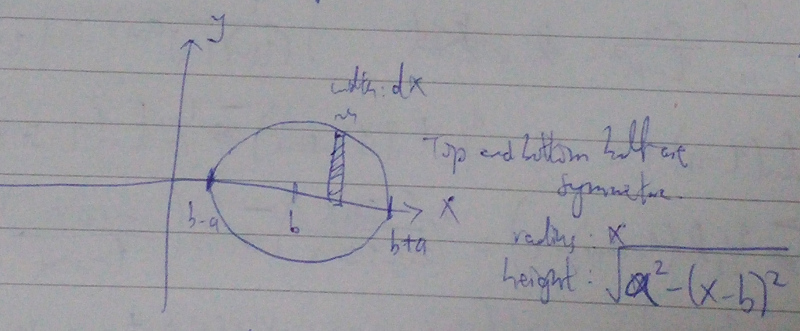
\includegraphics[scale=0.5]{q2.jpg}
\end{center}

For a circle centered at $x = b, y = 0$ with radius $a$, the volume of the torus is:

\begin{align*}
  2 \int_{b-a}^{b+a} 2 \pi x (\sqrt{a^2 - (x - b)^2}) dx &= 4 \pi \int_{b-a}^{b+a} x \sqrt{a^2 - (x - b)^2} dx
\end{align*}

Let $u = x - b$. Then $du = dx$. Also, $x = u + b$. Substitute those into the above:

\begin{align*}
  4 \pi \int_{b-a}^{b+a} x \sqrt{a^2 - (x - b)^2} dx &= 4 \pi \int_{-a}^{a} (u + b) \sqrt{a^2 - u^2} du \\
  &= 4 \pi (\int_{-a}^{a} u \sqrt{a^2 - u^2} du + b \int_{-a}^{a} \sqrt{a^2 - u^2} du) \\
  &= 4\pi ( -\frac{1}{2} \cdot \frac{({a^2 - u^2})^{3/2}}{\frac{3}{2}} \bigg]_{-a}^{a} + b \int_{-a}^{a} \sqrt{a^2 - u^2} du ) \\
  &= 4 \pi b \int_{-a}^{a} \sqrt{a^2 - u^2} du \ \ \ \ \text{(area of semicircle of radius $a$ centered at origin)} \\
  &= 4 \pi b (\frac{1}{2} \pi a^2) \\
  &= 2 \pi^2 a^2 b
\end{align*}


\begin{tcolorbox}
  \textbf{Q3a)} For any integer $n \geq 0$, use the substitution $tan^2 x = sec^2 x - 1$ to show that \\
  \begin{center}
    $\int tan^{n+2} x \ dx = \frac{1}{n + 1} tan^{n+1} x - \int tan^n x \ dx$
  \end{center}
\end{tcolorbox}

\begin{align*}
  \int tan^{n+2} x \ dx &= \int tan^2 x \ tan^n x \ dx \\
  &= \int (sec^2 x - 1) tan^n x \ dx \\
  &= \int sec^2 x \ tan^n x - tan^n x \ dx \\
  &= \frac{tan^{n+1} x}{n + 1} - \int tan^n x \ dx
\end{align*}


\begin{tcolorbox}
  \textbf{Q3b)} Deduce a formula for $\int tan^4 x \ dx$
\end{tcolorbox}

\begin{align*}
  \int tan^4 x \ dx &= \int tan^{2+2} x \ dx \\
  &= \frac{1}{2 + 1} tan^{2+1} x - \int tan^2 x \ dx \\
  &= \frac{1}{3} tan^3 x - \int tan^{0+2} x \ dx \\
  &= \frac{1}{3} tan^3 x - (\frac{1}{0+1} tan^{0+1} x - \int tan^0 x \ dx \\
  &= \frac{1}{3} tan^3 x - tan \ x + \int 1 dx \\
  &= \frac{1}{3} tan^3 x - tan \ x + x + C
\end{align*}

Verify:

\begin{align*}
  \frac{d}{dx}(\frac{1}{3} tan^3 x - tan \ x + x + C) &= tan^2 x \ sec^2 x - sec^2 x + 1 \\
  &= tan^2 x (1 + tan^2 x) - (1 + tan^2 x ) + 1 \\
  &= tan^2 x + tan^4 x - 1 - tan^2 x + 1 \\
  &= tan^4 x
\end{align*}


\begin{tcolorbox}
  \textbf{Q4a)} Derive a formula for $\int sec \ x \ dx$ by writing $sec \ x = \frac{cos \ x}{1 - sin^2 x}$ (verify this), and then making a substitution for $sin x$ and using partial fractions. (Your final answer must be expressed in terms of $x$.)
\end{tcolorbox}


\begin{align*}
  \frac{cos \ x}{1 - sin^2 x} &= \frac{cos \ x}{cos^2 x} \\
  &= \frac{1}{cos \ x} \\
  &= sec \ x
\end{align*}

For $\int sec x \ dx = \int \frac{cos \ x}{1 - sin^2 x} dx$, let $u = sin x$. Then $du = cos \ x \ dx$

\begin{align*}
  \frac{cos \ x}{1 - sin^2 x} dx &= \int \frac{du}{1 - u^2} \\
  &= \int \frac{1}{(1 + u)(1 - u)} du \\
  &= \int \frac{1 / 2}{1 + u} + \frac{1 / 2}{1 - u} du \\
  &= \frac{1}{2} ln(1 + u) - \frac{1}{2} ln(1 - u) + C \\
  &= \frac{1}{2} ln(1 + sin \ x) - \frac{1}{2} ln(1 - sin \ x) + C \\
\end{align*}

Verify:

\begin{align*}
  \frac{1}{2} ln(1 + sin \ x) - \frac{1}{2} ln(1 - sin \ x) + C &= \frac{1}{2} (\frac{cos \ x}{1 + sin \ x}) - \frac{1}{2} (\frac{- cos \ x}{1 - sin x}) \\
  &= \frac{1}{2} (\frac{cos \ x (1 - sin \ x) + cos \ x (1 + sin \ x)}{(1 + sin \ x)(1 - sin \ x)}) \\
  &= \frac{1}{2} (\frac{cos \ x - sin \ x \ cos \ x + cos \ x + sin \ x \ cos \ x}{1 - sin^2 x}) \\
  &= \frac{1}{2} (\frac{2 cos \ x}{cos^2 x}) \\
  &= \frac{1}{cos \ x} \\
  &= sec \ x
\end{align*}


\begin{tcolorbox}
  \textbf{Q4b)} Convert the formula into the more familiar one by multiplying the fraction in the answer on both top and bottom by $1 + sin \ x$. (Note that $(1 / 2) ln \ u = ln \sqrt{u}$
\end{tcolorbox}

\begin{align*}
  \frac{1}{2} ln(1 + sin \ x) - \frac{1}{2} ln(1 - sin \ x) + C &= \frac{1}{2} (ln(1 + sin \ x) - ln(1 - sin \ x)) \\
  &= \frac{1}{2} ln(\frac{1 + sin \ x}{1 - sin \ x}) \\
  &= \frac{1}{2} ln(\frac{1 + sin \ x}{1 - sin \ x} \cdot \frac{1 + sin \ x}{1 + sin \ x}) \\
  &= \frac{1}{2} ln(\frac{sin^2 x + 2 sin \ x + 1}{1 - sin^2 x}) \\
  &= \frac{1}{2} ln(\frac{sin^2 x + 2 sin \ x + 1}{cos^2 x}) \\
  &= \frac{1}{2} ln(\frac{sin^2 x}{cos^2 x} + \frac{2 sin \ x}{cos^2 x} + \frac{1}{cos^2 x}) \\
  &= \frac{1}{2} ln(tan^2 x + 2 sec \ x \ tan \ x + sec^2 x) \\
  &= \frac{1}{2} ln((sec \ x + tan \ x)^2) \\
  &= ln(\sqrt{(sec \ x + tan \ x)^2}) \\
  &= ln(sec \ x + tan \ x)
\end{align*}

\end{document}
